% lint-skip: 未完成ステータス（figure/table caption 未対応，人手チェック時に解消予定）
\documentclass[../../main.tex]{subfiles}
\begin{document}

\begin{flushright}
  \footnotesize\textit{【自動文字起こし・要確認】}
\end{flushright}

{\bf [解答]} 正四面体の一辺の長さを1として良い．座標空間において，
$$A\left(0, 0, \dfrac{\sqrt{6}}{3}\right),\ B\left(\dfrac{\sqrt{3}}{3}, 0, 0\right)$$
$$C\left(-\dfrac{\sqrt{3}}{6}, \dfrac{1}{2}, 0\right),\ D\left(-\dfrac{\sqrt{3}}{6}, -\dfrac{1}{2}, 0\right)$$
とおける．すると $B, C, D$ を通る円は $z=0, x^2+y^2 = \dfrac{1}{3}$ である．

\begin{figure}[htbp]
  \centering
  \begin{minipage}{0.47\linewidth}
    \centering
    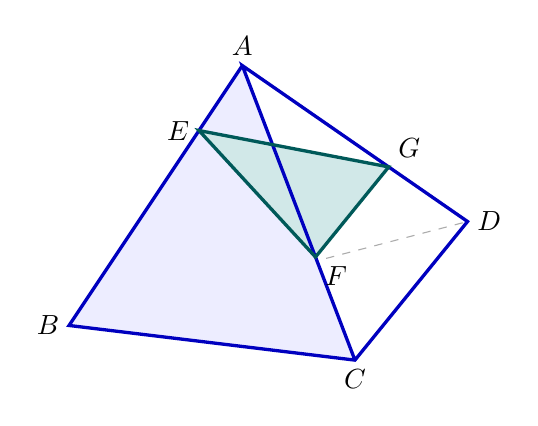
\begin{tikzpicture}[scale=1.1]
      % s=1/4，t=13/20 の代表図。
      \coordinate (A) at (0,3);
      \coordinate (B) at (-2,0);
      \coordinate (C) at (1.3,-0.4);
      \coordinate (D) at (2.6,1.2);
      \coordinate (E) at (-0.5,2.25);
      \coordinate (F) at (0.845,0.79);
      \coordinate (G) at (1.69,1.83);
      \draw[dashed,gray!65] (B)--(D);
      \fill[blue!7] (A)--(B)--(C)--cycle;
      \fill[teal!18] (E)--(F)--(G)--cycle;
      \draw[blue!75!black,very thick] (A)--(B)--(C)--(D)--(A)--(C);
      \draw[teal!70!black,very thick] (E)--(F)--(G)--cycle;
      \node[above] at (A) {$A$};
      \node[left] at (B) {$B$};
      \node[below] at (C) {$C$};
      \node[right] at (D) {$D$};
      \node[left] at (E) {$E$};
      \node[below right] at (F) {$F$};
      \node[above right] at (G) {$G$};
    \end{tikzpicture}
  \end{minipage}\hfill
  \begin{minipage}{0.49\linewidth}
    \centering
    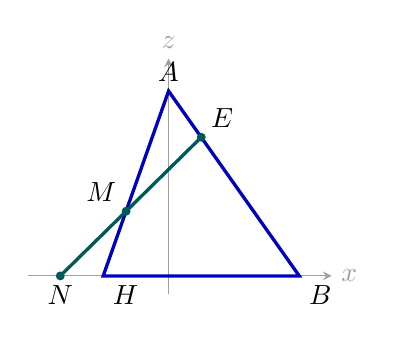
\begin{tikzpicture}[scale=1.15,>=stealth]
      % 同じ s,t を xz 平面に射影した断面。
      \coordinate (A) at (0,2.041);
      \coordinate (B) at (1.443,0);
      \coordinate (H) at (-0.722,0);
      \coordinate (E) at (0.361,1.531);
      \coordinate (M) at (-0.469,0.714);
      \coordinate (N) at (-1.196,0);
      \draw[->,gray!75] (-1.55,0)--(1.8,0) node[right] {$x$};
      \draw[->,gray!75] (0,-0.2)--(0,2.4) node[above] {$z$};
      \draw[blue!75!black,very thick] (A)--(H)--(B)--cycle;
      \draw[teal!70!black,very thick] (N)--(M)--(E);
      \fill[teal!70!black] (E) circle (1.4pt) (M) circle (1.4pt) (N) circle (1.4pt);
      \node[above] at (A) {$A$};
      \node[below right] at (B) {$B$};
      \node[below right] at (H) {$H$};
      \node[above right] at (E) {$E$};
      \node[above left] at (M) {$M$};
      \node[below] at (N) {$N$};
    \end{tikzpicture}
  \end{minipage}
  \caption{正四面体と切断面，および $xz$ 平面で見た点 $E,M,N,H$}
\end{figure}

$xz$平面で立体を切断すると左下図で線分$FG$の中点を$M$とし，
$EM$と$xy$平面の交点を$N$，$AM$と$x$軸の交点を$H$とすると，メネラウスの定理から
$$\dfrac{1-s}{s} \cdot \dfrac{NH}{BN} \cdot \dfrac{t}{1-t} = 1$$
$$BN = \dfrac{1-s}{s} \dfrac{t}{1-t} NH$$
だから $NH = p$ として，
$$\left(\dfrac{\sqrt{3}}{2} + p\right) = \dfrac{1-s}{s} \dfrac{t}{1-t} p$$
$$\therefore p = \dfrac{\dfrac{\sqrt{3}}{2}}{\dfrac{1-s}{s}\dfrac{t}{1-t} - 1} \quad (>0)$$
だから，$N\left(-\dfrac{\sqrt{3}}{6} - p, 0, 0\right)$ である．図形の対称性から，条件は
$$-\dfrac{\sqrt{3}}{6} - p \ge -\dfrac{\sqrt{3}}{3} \quad (\because ON \le \text{円の半径})$$
$$\Leftrightarrow 4s(1-t) \le (1-s)t \quad \left(\because p>0 \text{から} \dfrac{1-s}{s}\dfrac{t}{1-t} > 1 \Leftrightarrow t > s\right)$$
これと $0 < t, s < 1$ を図示して，下図（境界は $t = \dfrac{4s}{1+3s}$ のみ含む）

\begin{figure}[H]
  \centering
  \begin{tikzpicture}[x=4cm,y=4cm,>=stealth]
    \fill[teal!16] (0,1)--(1,1)
    -- plot[domain=1:0,samples=100] (\x,{4*\x/(1+3*\x)}) -- cycle;
    \draw[->,gray!75] (-0.08,0)--(1.17,0) node[right] {$s$};
    \draw[->,gray!75] (0,-0.08)--(0,1.17) node[above] {$t$};
    \draw[dashed,gray!70] (1,0)--(1,1)--(0,1);
    \draw[dashed,gray!55] (0,0)--(1,1);
    \draw[teal!70!black,very thick,domain=0.008:0.992,samples=100]
    plot (\x,{4*\x/(1+3*\x)});
    \fill[white,draw=teal!70!black,thick] (0,0) circle (1.4pt)
    (1,1) circle (1.4pt);
    \node[below] at (1,0) {$1$};
    \node[left] at (0,1) {$1$};
    \node[teal!70!black,below right] at (0.47,0.63)
    {$t=\frac{4s}{1+3s}$};
    \node at (0.43,0.91) {条件を満たす領域};
  \end{tikzpicture}
  \caption{$0<s,t<1$ における許容範囲．曲線上を含み，外枠は含まない}
\end{figure}

\end{document}
